\documentclass{article}

\usepackage{graphicx}
\usepackage{tikz}
\usepackage{tikzsymbols}
\usetikzlibrary{calc,patterns,shapes.geometric}
\pagestyle{empty}
\usepackage[margin=0pt]{geometry}
\geometry{papersize={14in,12in}}

\def\centerarc[#1](#2)(#3:#4:#5){\draw[#1] ($(#2)+({#5*cos(#3)},{#5*sin(#3)})$) arc (#3:#4:#5);}

\begin{document}
	\begin{figure}
		\centering
		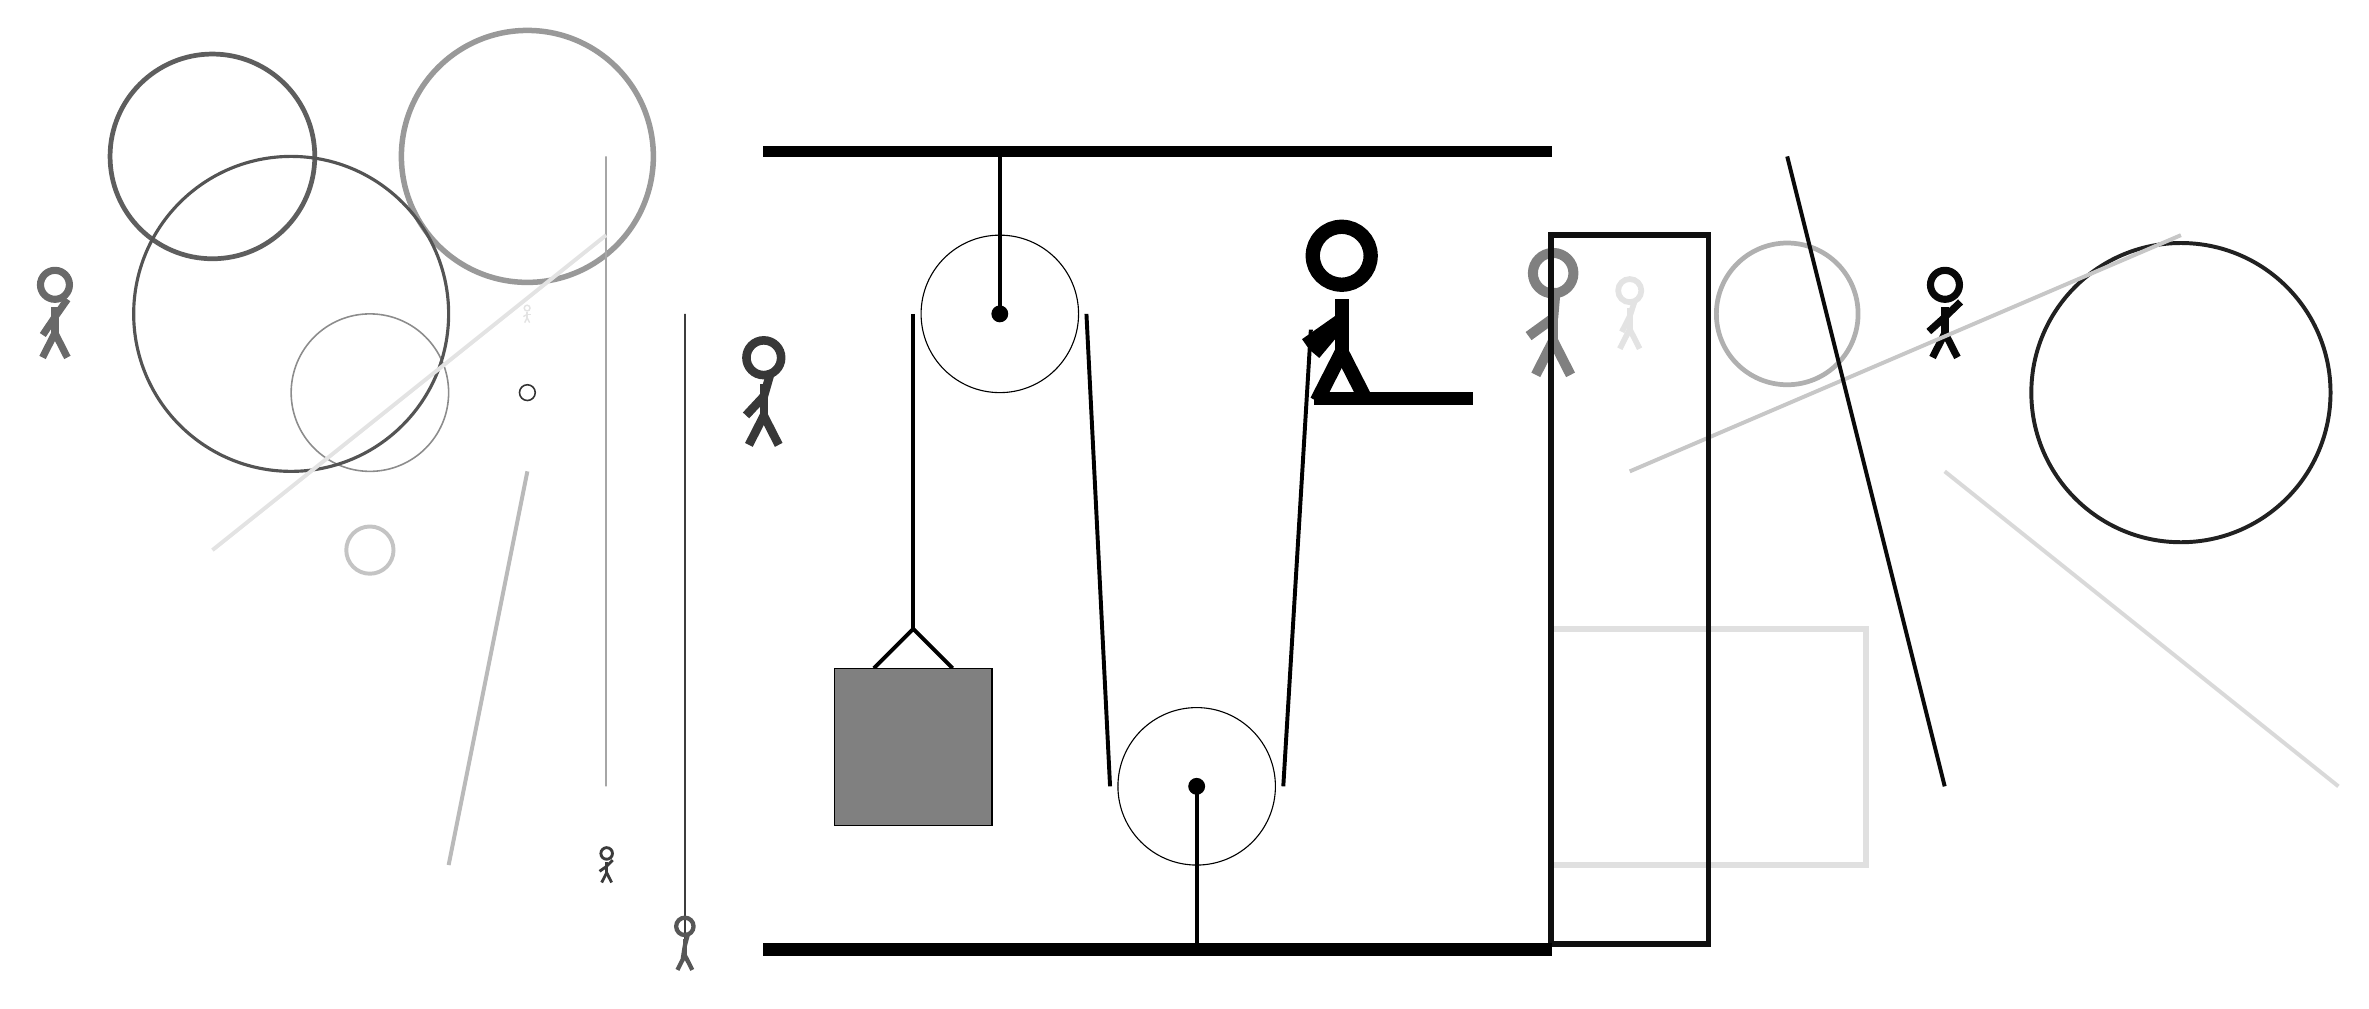
\begin{tikzpicture}
			%%%%% START %%%%%
			
			\draw[fill=black] (-2, 10) rectangle (8, 10.125);
			
			\draw (3.5, 2.0) circle (1);
			\draw[fill=black] (3.5, 2.0) circle (0.1);
			\draw[line width=0.5mm] (3.5, 2.0) -- (3.5, 0);
			
			\draw (1, 8) circle (1);
			\draw[fill=black] (1, 8) circle (0.1);
			\draw[line width=0.5mm] (1, 10) -- (1, 8);
			
			\node[line width=0.5mm, color=black!11] at (9, 8) {\Strichmaxerl[4][63][72]};
			
			\draw [line width=0.2mm, color=black!67](-2, 3) circle (0.0);
			\draw[line width=0.5mm, color=black!27](-5, 6) -- (-6, 1);
			\draw [line width=0.2mm, color=black!45](-7, 7) circle (1.0);
			\node[line width=0.4mm, color=black!97] at (13, 8) {\Strichmaxerl[5][42][44]};
			
			\draw[line width=0.5mm, color=black!15](13, 6) -- (18, 2);
			\node[line width=0.2mm, color=black!11] at (-5, 8) {\Strichmaxerl[1][28][0]};
			
			\node[line width=0.2mm, color=black!78] at (-2, 7) {\Strichmaxerl[6][47][74]};
			\draw [line width=0.5mm, color=black!87](16, 7) circle (1.9);
			
			\node[line width=0.3mm, color=black!50] at (8, 8) {\Strichmaxerl[7][36][85]};
			\draw[line width=0.5mm, color=black!22](9, 6) -- (16, 9);
			
			\draw [line width=0.6mm, color=black!31](11, 8) circle (0.9);
			\draw [line width=0.2mm, color=black!80](-5, 7) circle (0.1);
			
			\draw[line width=0.7mm, color=black!12] (8, 4) rectangle (12, 1);
			\draw [line width=0.5mm, color=black!23](-7, 5) circle (0.3);
			\draw[line width=0.5mm, color=black!96](13, 2) -- (11, 10);
			
			\node[line width=0.2mm, color=black!77] at (-4, 1) {\Strichmaxerl[2][35][46]};
			\draw [line width=0.7mm, color=black!40](-5, 10) circle (1.6);
			\draw[line width=0.2mm, color=black!35] (-4, 10) rectangle (-4, 2);
			
			\draw[line width=0.3mm, color=black!76] (-3, 0) rectangle (-3, 8);
			\draw [line width=0.6mm, color=black!63](-9, 10) circle (1.3);
			\draw [line width=0.4mm, color=black!67](-8, 8) circle (2.0);
			
			\node[line width=0.5mm, color=black!59] at (-11, 8) {\Strichmaxerl[5][56][55]};
			\draw[line width=0.5mm, color=black!11](-4, 9) -- (-9, 5);
			\node[line width=0.6mm, color=black!66] at (-3, 0) {\Strichmaxerl[3][81][75]};
			
			\draw[line width=0.7mm, color=black!94] (10, 0) rectangle (8, 9);
			
			
			\draw[line width=0.5mm](-0.6, 3.5) --  (-0.1, 4.0) -- (0.4, 3.5);
			\draw[fill=black!50] (-1.1, 3.5) rectangle (0.9, 1.5);
			
			\draw[line width=0.5mm](-0.1, 8) -- (-0.1, 4.0);
			\centerarc[line width=0.5mm](1, 8)(180:0:1.1)
			\draw[line width=0.5mm](2.1, 8) -- (2.4, 2.0);
			\centerarc[line width=0.5mm](3.5, 2.0)(180:360:1.1)
			\draw[line width=0.5mm](4.6, 2.0) -- (4.95, 7.8);
			
			\node at (5.3, 8) {\Strichmaxerl[10][35][-130]};
			\draw[fill=black] (5, 7) rectangle (7, 6.85);
			
			\draw[fill=black] (-2, 0) rectangle (8, -0.15);
			
			%%%%% END %%%%%
		\end{tikzpicture}
	\end{figure}	
\end{document}